%%%%%%%%%%%%%%%%%%%%%%%%%%%%%%%%%%%%%%%%%%%%%%%%
\section{Introduction}


%%%%%%%%%%%%%%%%%%%%%%%%%%%%%%%%%%%%%%%%%%%%%%%%%%%
\begin{frame}

\frametitle{Overview}

Snakemake is:
\begin{itemize}
  \item a workflow engine based on Python
  \item useful for applying a series of commands (i.e., a ``pipeline'')
\end{itemize}

\pause

\begin{figure}
  \centering
  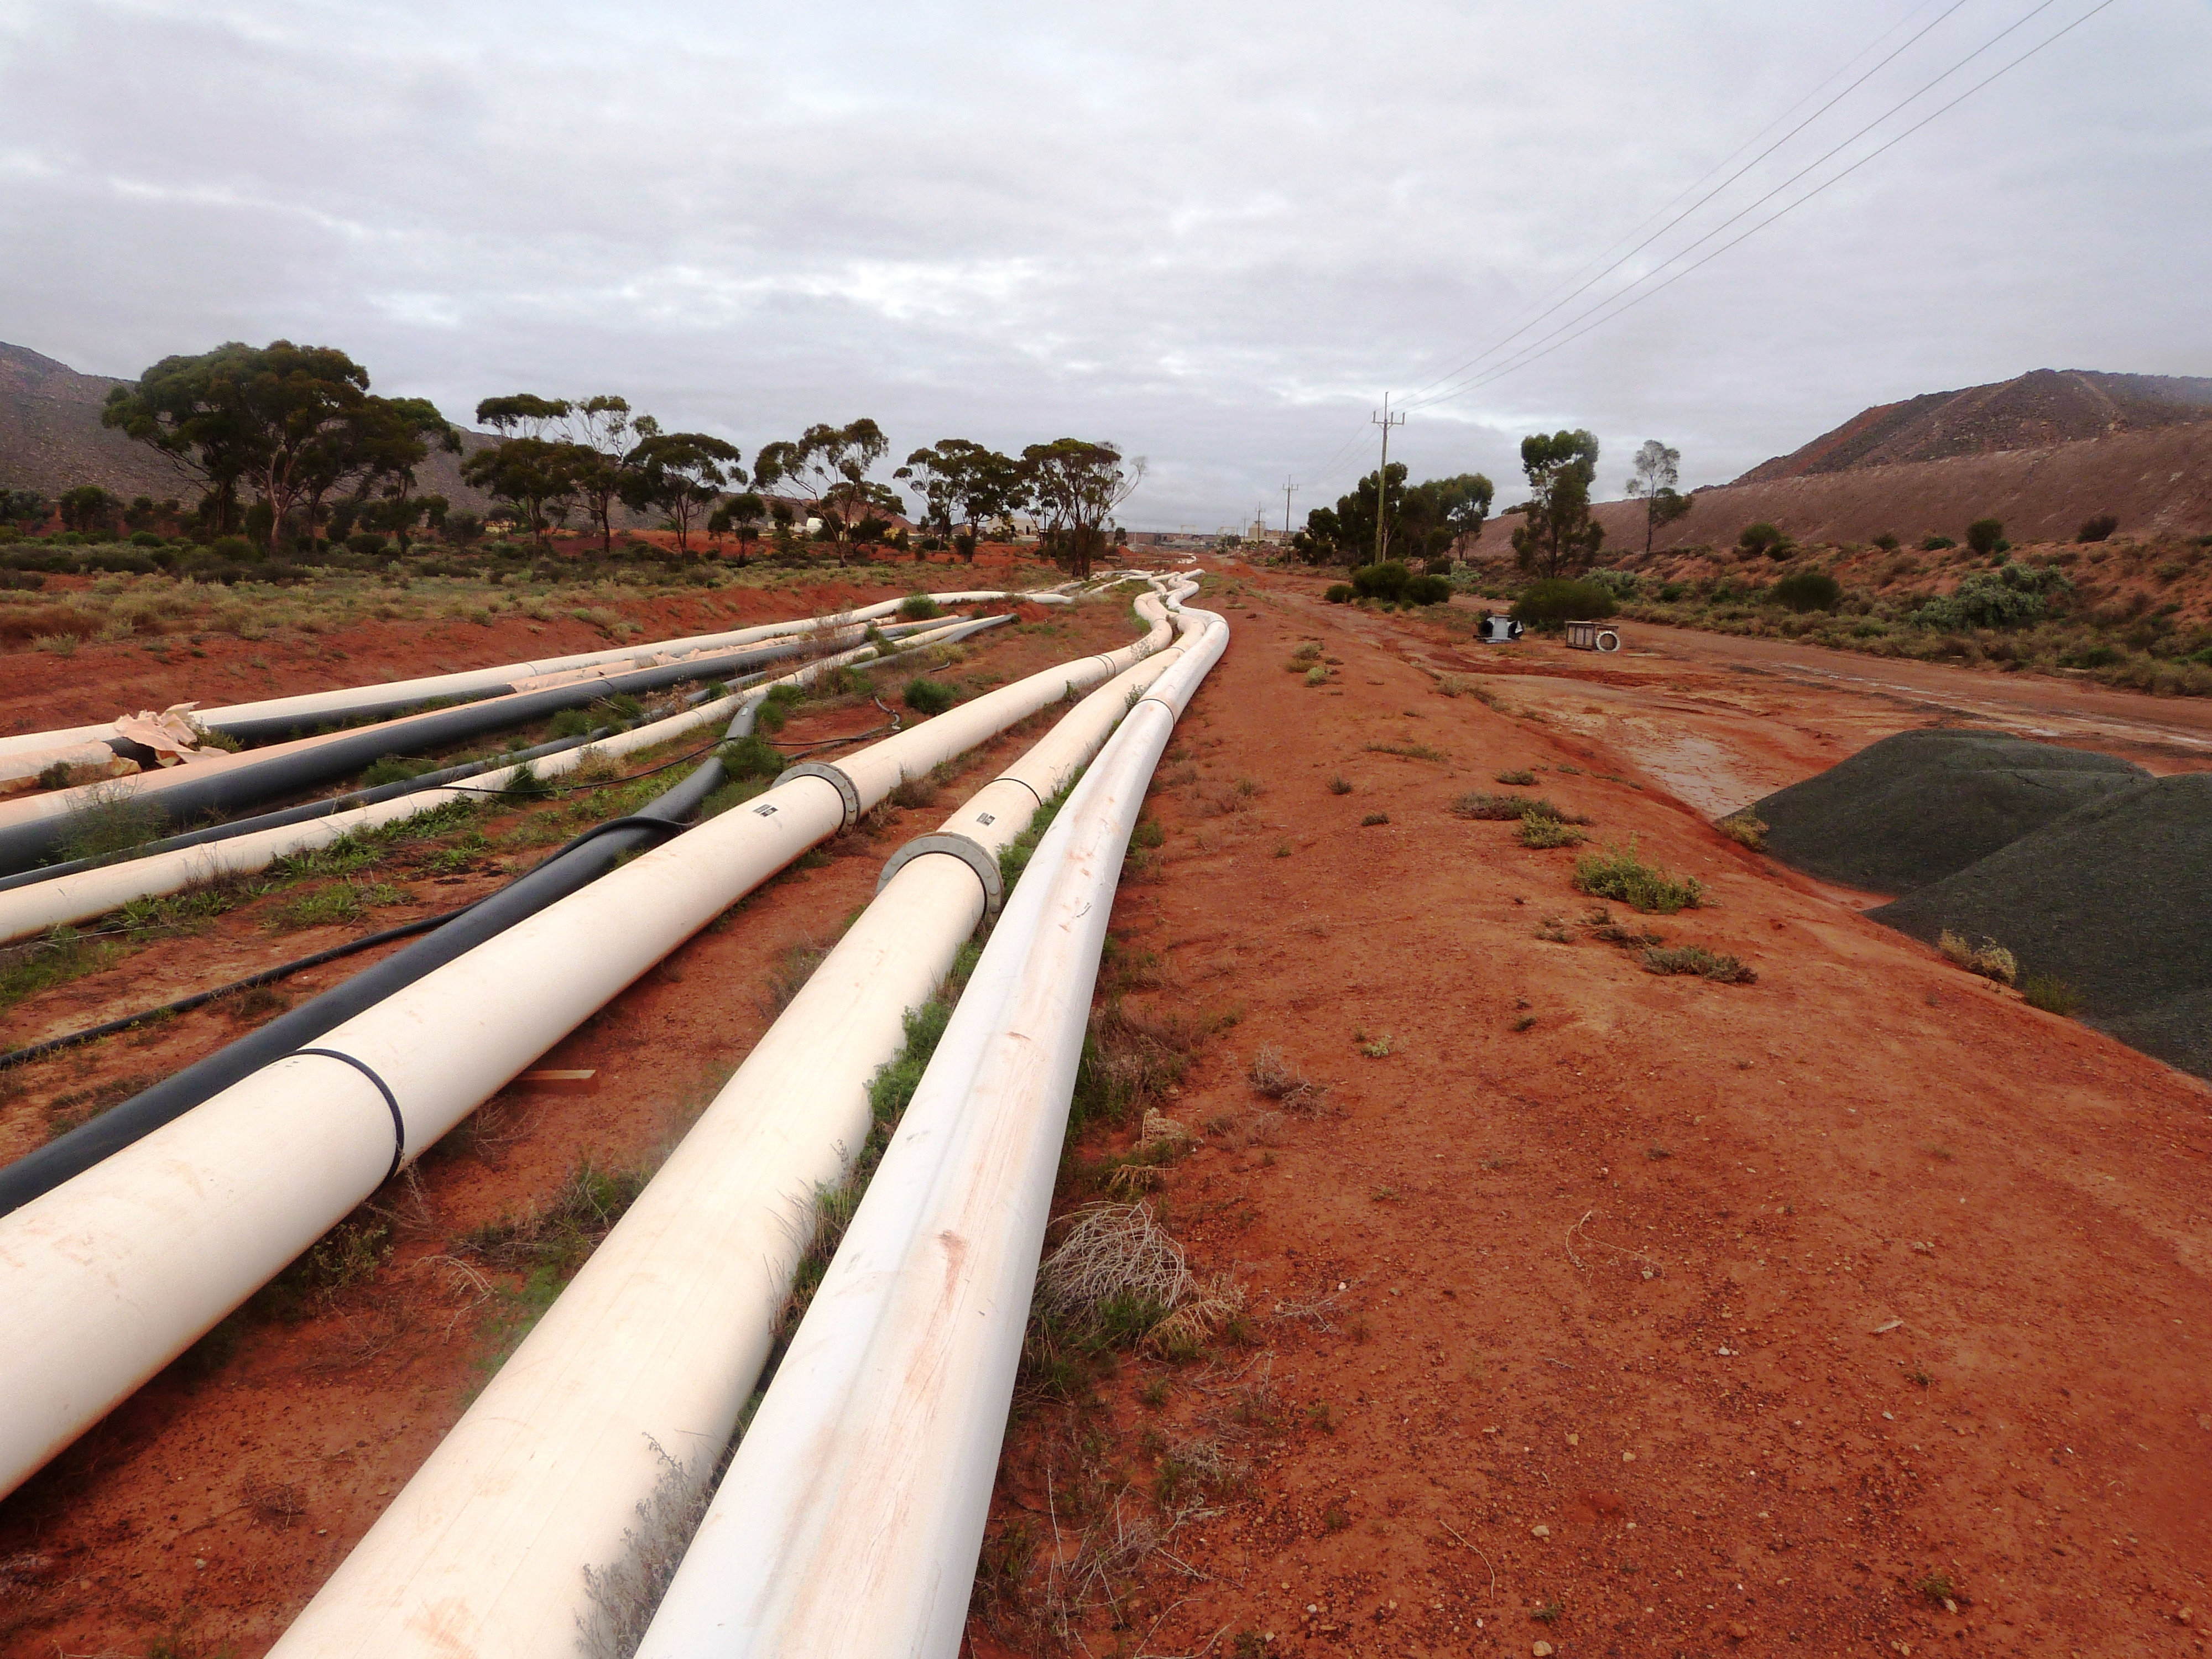
\includegraphics[width=5cm]{intro/pipeline}
\end{figure}

{\figsource{Wikipedia:  pipeline}}

\end{frame}


%%%%%%%%%%%%%%%%%%%%%%%%%%%%%%%%%%%%%%%%%%%%%%%%%%%
\begin{frame}

\frametitle{Overview}

\begin{figure}
  \centering
  
\includegraphics[width=\linewidth]{intro/kr12-bio-cover}
\end{figure}

\pause

\begin{figure}
  \centering
  {\fbox{
\includegraphics[width=8cm]{intro/snakemake-citations}}}
\end{figure}

\figsource{\citep{kr12:bio}}

\end{frame}


%%%%%%%%%%%%%%%%%%%%%%%%%%%%%%%%%%%%%%%%%%%%%%%%%%%
\begin{frame}

\frametitle{Overview}

Currently, Snakemake developers encouraging citing this ``rolling'' publication:
\begin{figure}
  \centering
  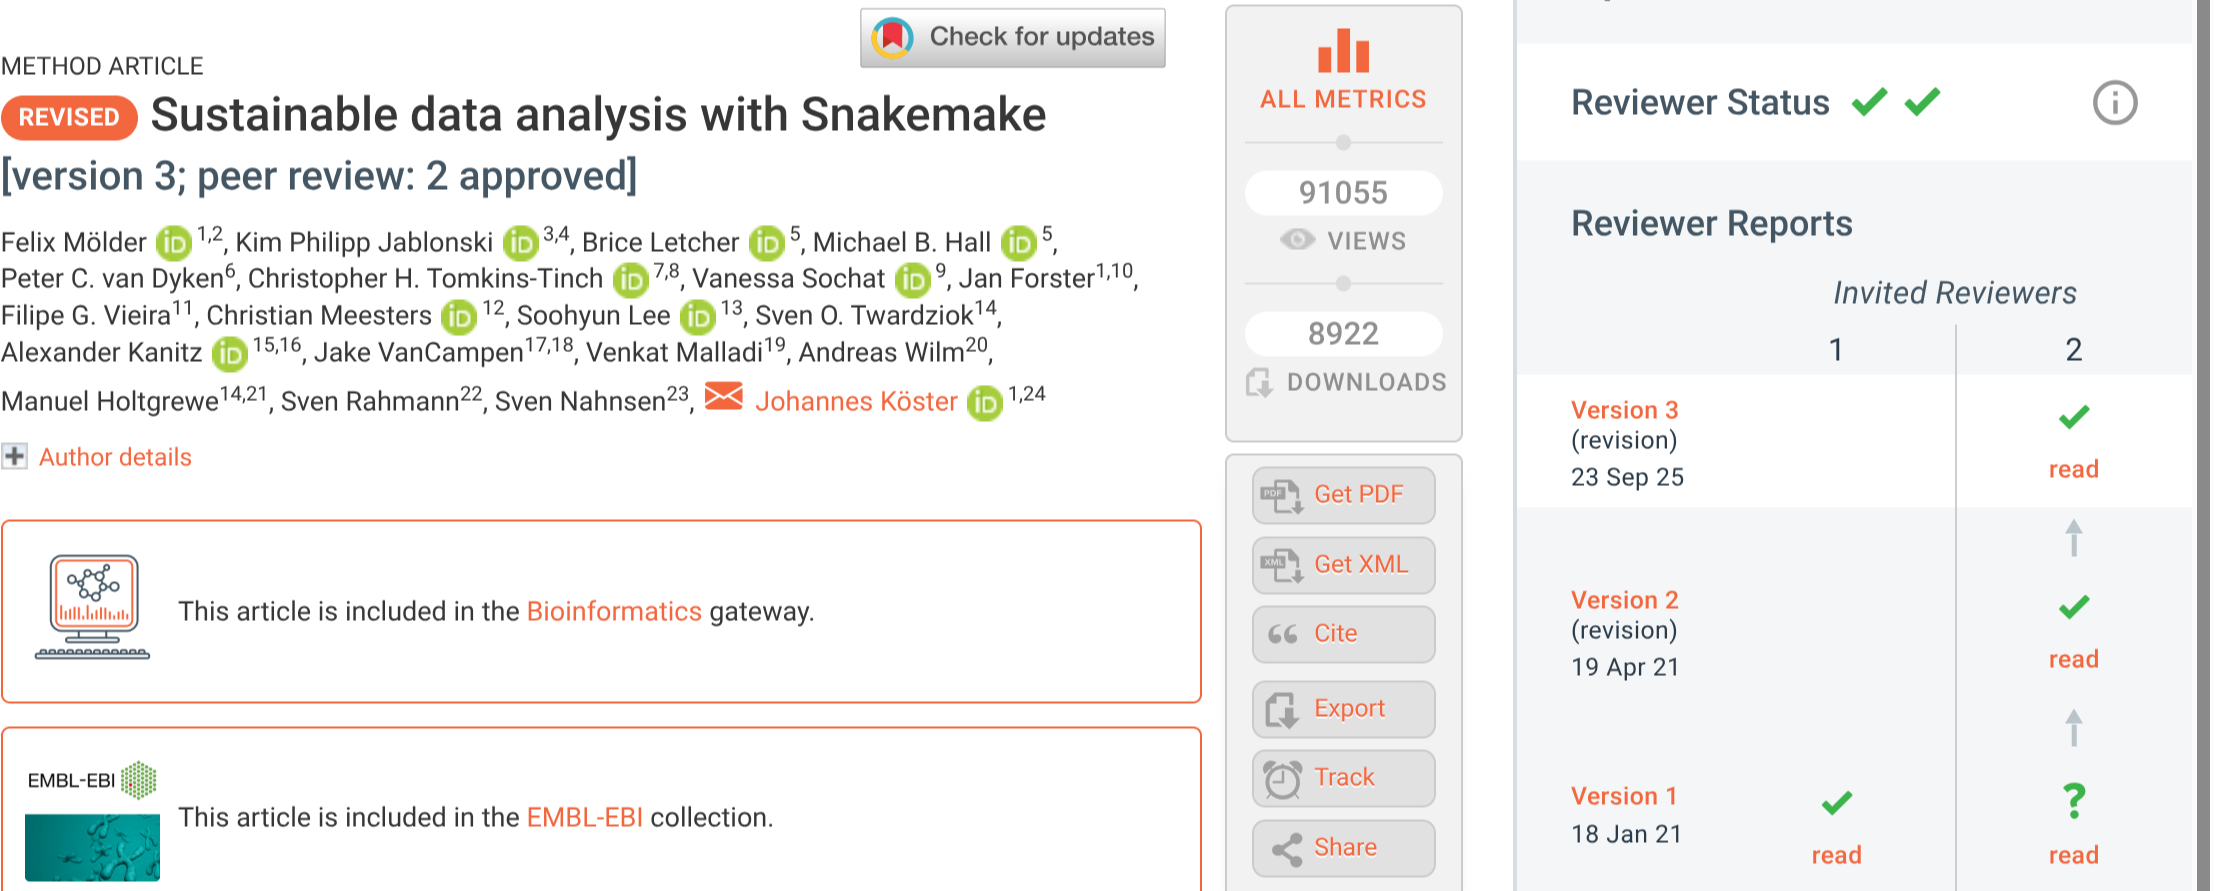
\includegraphics[width=\linewidth]{intro/mjlhv25-f1000-cover}
\end{figure}

\figsource{\citep{mjlhv25:f1000}}

\end{frame}


%%%%%%%%%%%%%%%%%%%%%%%%%%%%%%%%%%%%%%%%%%%%%%%%%%%
\begin{frame}

\frametitle{Snakemake's homepage}

\begin{figure}
  \centering
  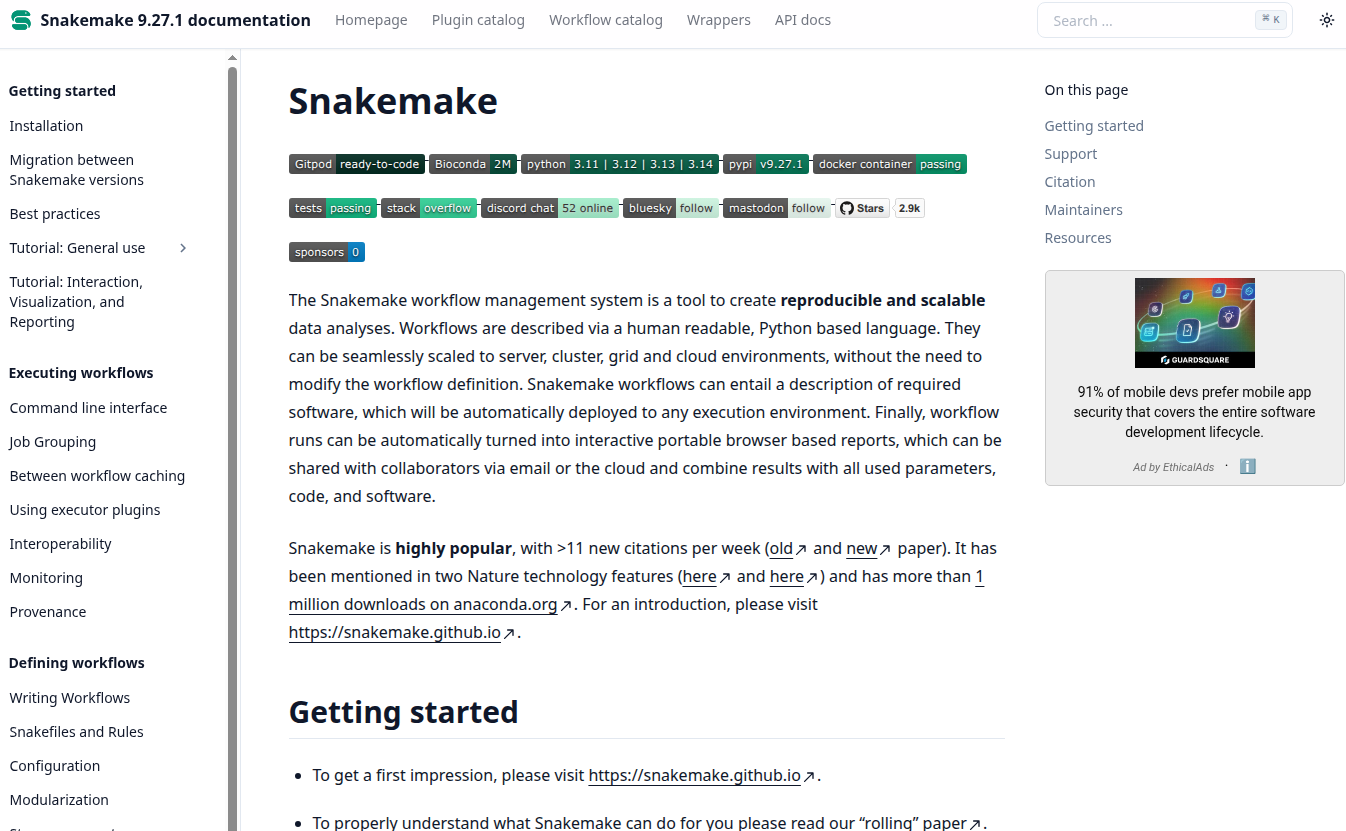
\includegraphics[height=6cm]{intro/snakemake-homepage}
\end{figure}

{\figsource{\href{https://snakemake.readthedocs.io/en/stable/}{https://snakemake.readthedocs.io/en/stable/}}}

\end{frame}


%%%%%%%%%%%%%%%%%%%%%%%%%%%%%%%%%%%%%%%%%%%%%%%%%%%
\begin{frame}

\frametitle{Snakemake's tutorial}

\begin{figure}
  \centering
  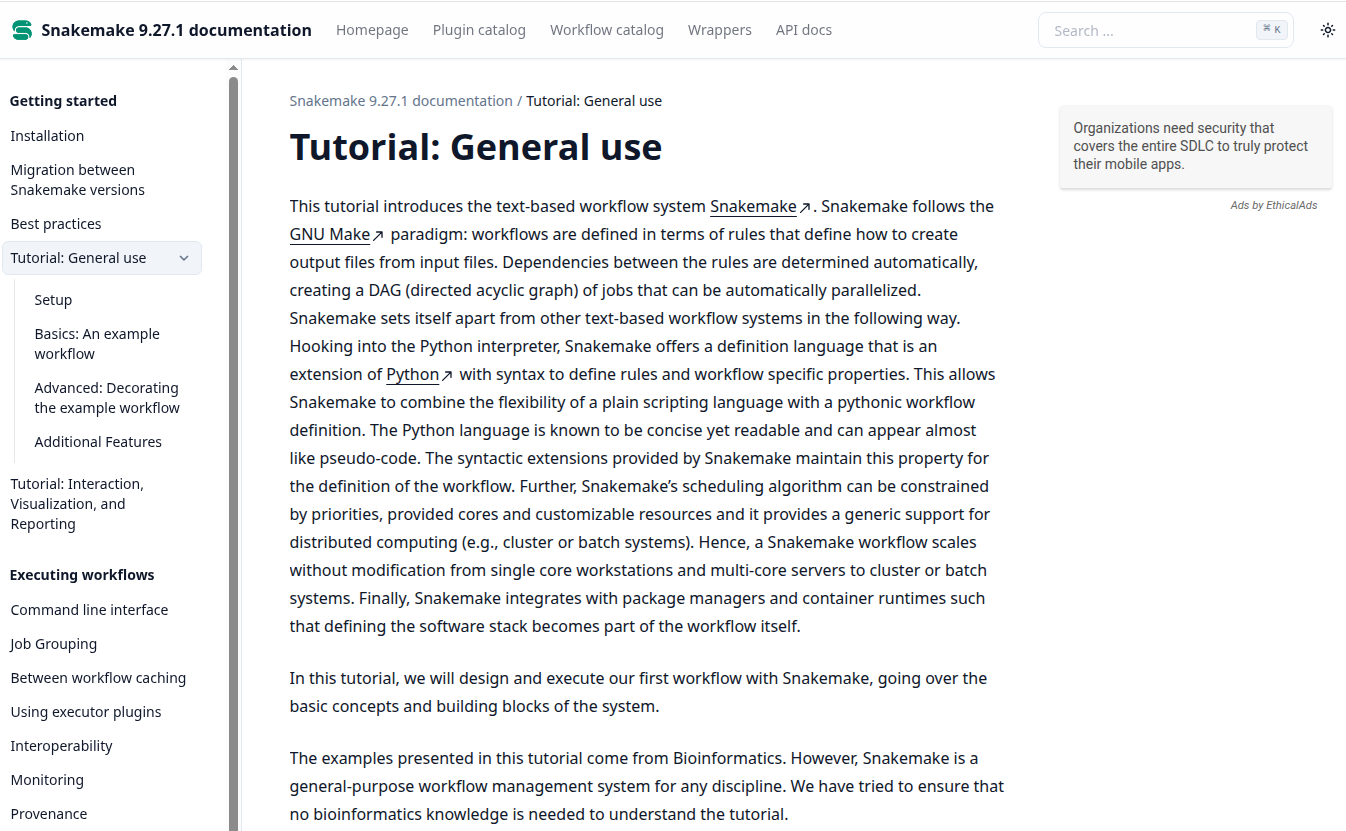
\includegraphics[height=6cm]{intro/snakemake-tutorial}
\end{figure}

{\figsource{\href{https://snakemake.readthedocs.io/en/stable/tutorial/tutorial.html}{https://snakemake.readthedocs.io/en/stable/tutorial/tutorial.html}}}

\end{frame}


%%%%%%%%%%%%%%%%%%%%%%%%%%%%%%%%%%%%%%%%%%%%%%%%%%%
\begin{frame}

\frametitle{YouTube videos}

\begin{figure}
  \centering
  {\fbox{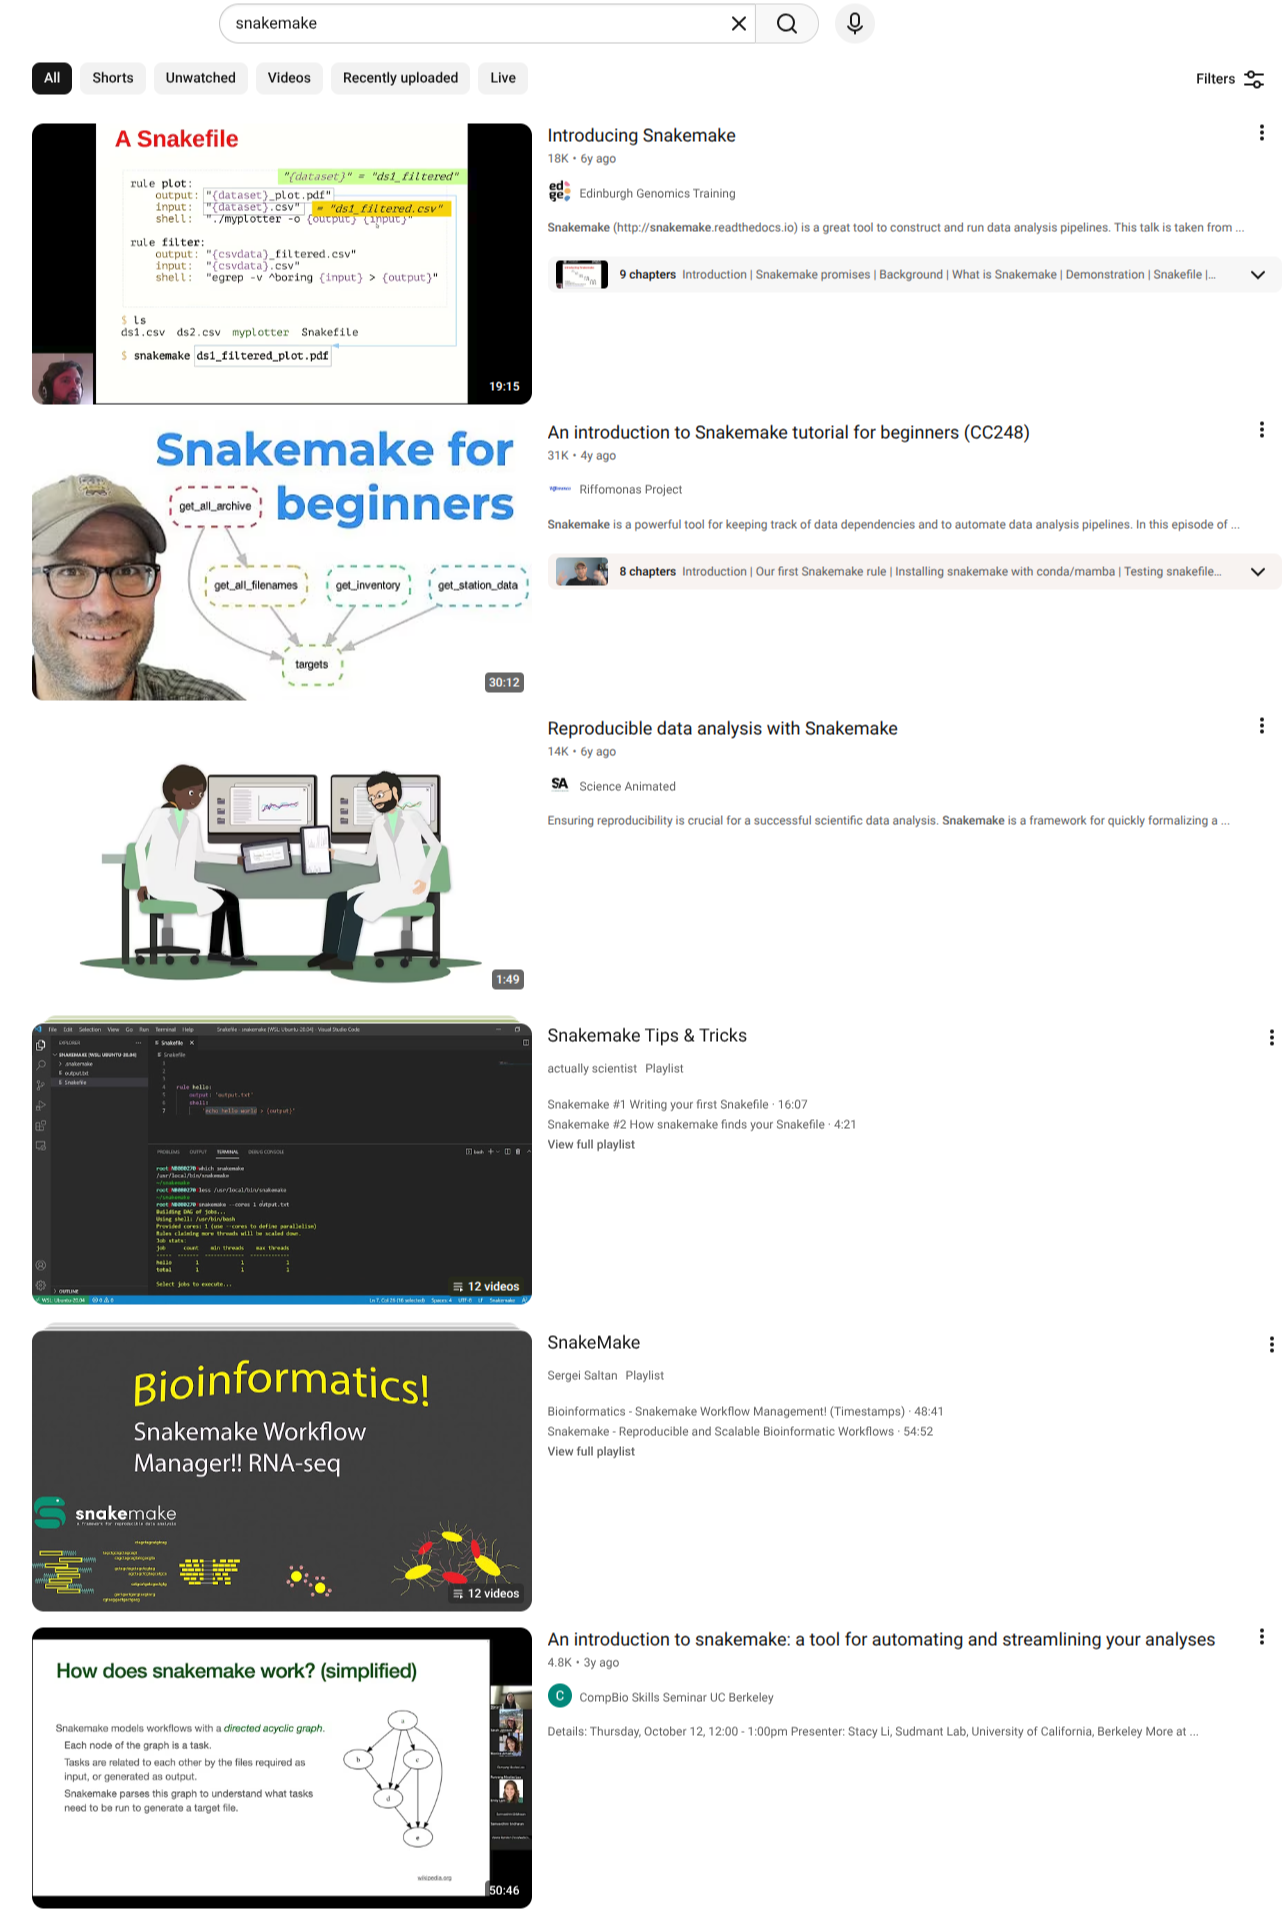
\includegraphics[height=5cm]{intro/youtube}}}
\end{figure}

So, a lot of information on the Internet now...

\end{frame}


%%%%%%%%%%%%%%%%%%%%%%%%%%%%%%%%%%%%%%%%%%%%%%%%%%%
\begin{frame}

\frametitle{My story}

By 2016, I had been working in bioinformatics for $>$10 years...
\begin{itemize}
  \item Quite stuck in my ways for workflows (i.e., {\texttt{bash}} scripts).
  \item A new colleague joined our lab with a background in CS.  Asked me where to start.  I had recently came across the Snakemake paper and gave it to him since he also knew Python.
  \item A fast learner, he picked it up in a week.  And he kept telling me how great it was.
  \item Months later, I switched, spending just over a week changing what I had been doing from {\texttt{bash}} to Snakemake.
\end{itemize}

Of course, one of the best decisions I have made as a bioinformatician...

\end{frame}


%%%%%%%%%%%%%%%%%%%%%%%%%%%%%%%%%%%%%%%%%%%%%%%%%%%
\begin{frame}

\frametitle{Talk's motivation}

Motivation of this talk:
\begin{itemize}
  \item I assume that you have a workflow / need to develop a workflow.
  \item There are so many languages and tools out there... \Smiles{-1.0}
  \item You are wondering if Snakemake is ``worth your time''...
\end{itemize}
\vs

Everything might be too fast today.  My aim is to provide a ``bird's eye'' view so that (hopefully) you have enough information to decide if you should invest more time.
\vs

If it is what you are looking for, then you have the Snakemake homepage, YouTube videos, etc. as your next resource.

\end{frame}


%%%%%%%%%%%%%%%%%%%%%%%%%%%%%%%%%%%%%%%%%%%%%%%%%%%
\begin{frame}

\frametitle{Talk's motivation}

``Disclaimer'':
\begin{itemize}
  \item Despite using it for 10 years, I only know what I needed.  I have not yet explored many (newer...) features about Snakemake.
  \item Have been happy with it since 2016; did not look into alternatives.  No doubt there are better alternatives out there!
\end{itemize}
\vs

Alternatives:
\begin{itemize}
  \item NextFlow
  \item Common Workflow Language (CWL)
  \item Galaxy (i.e., web browser based)
\end{itemize}

\end{frame}


%%%%%%%%%%%%%%%%%%%%%%%%%%%%%%%%%%%%%%%%%%%%%%%%%%%
\begin{frame}

\frametitle{Google trends}

\begin{figure}
  \centering
  {\fbox{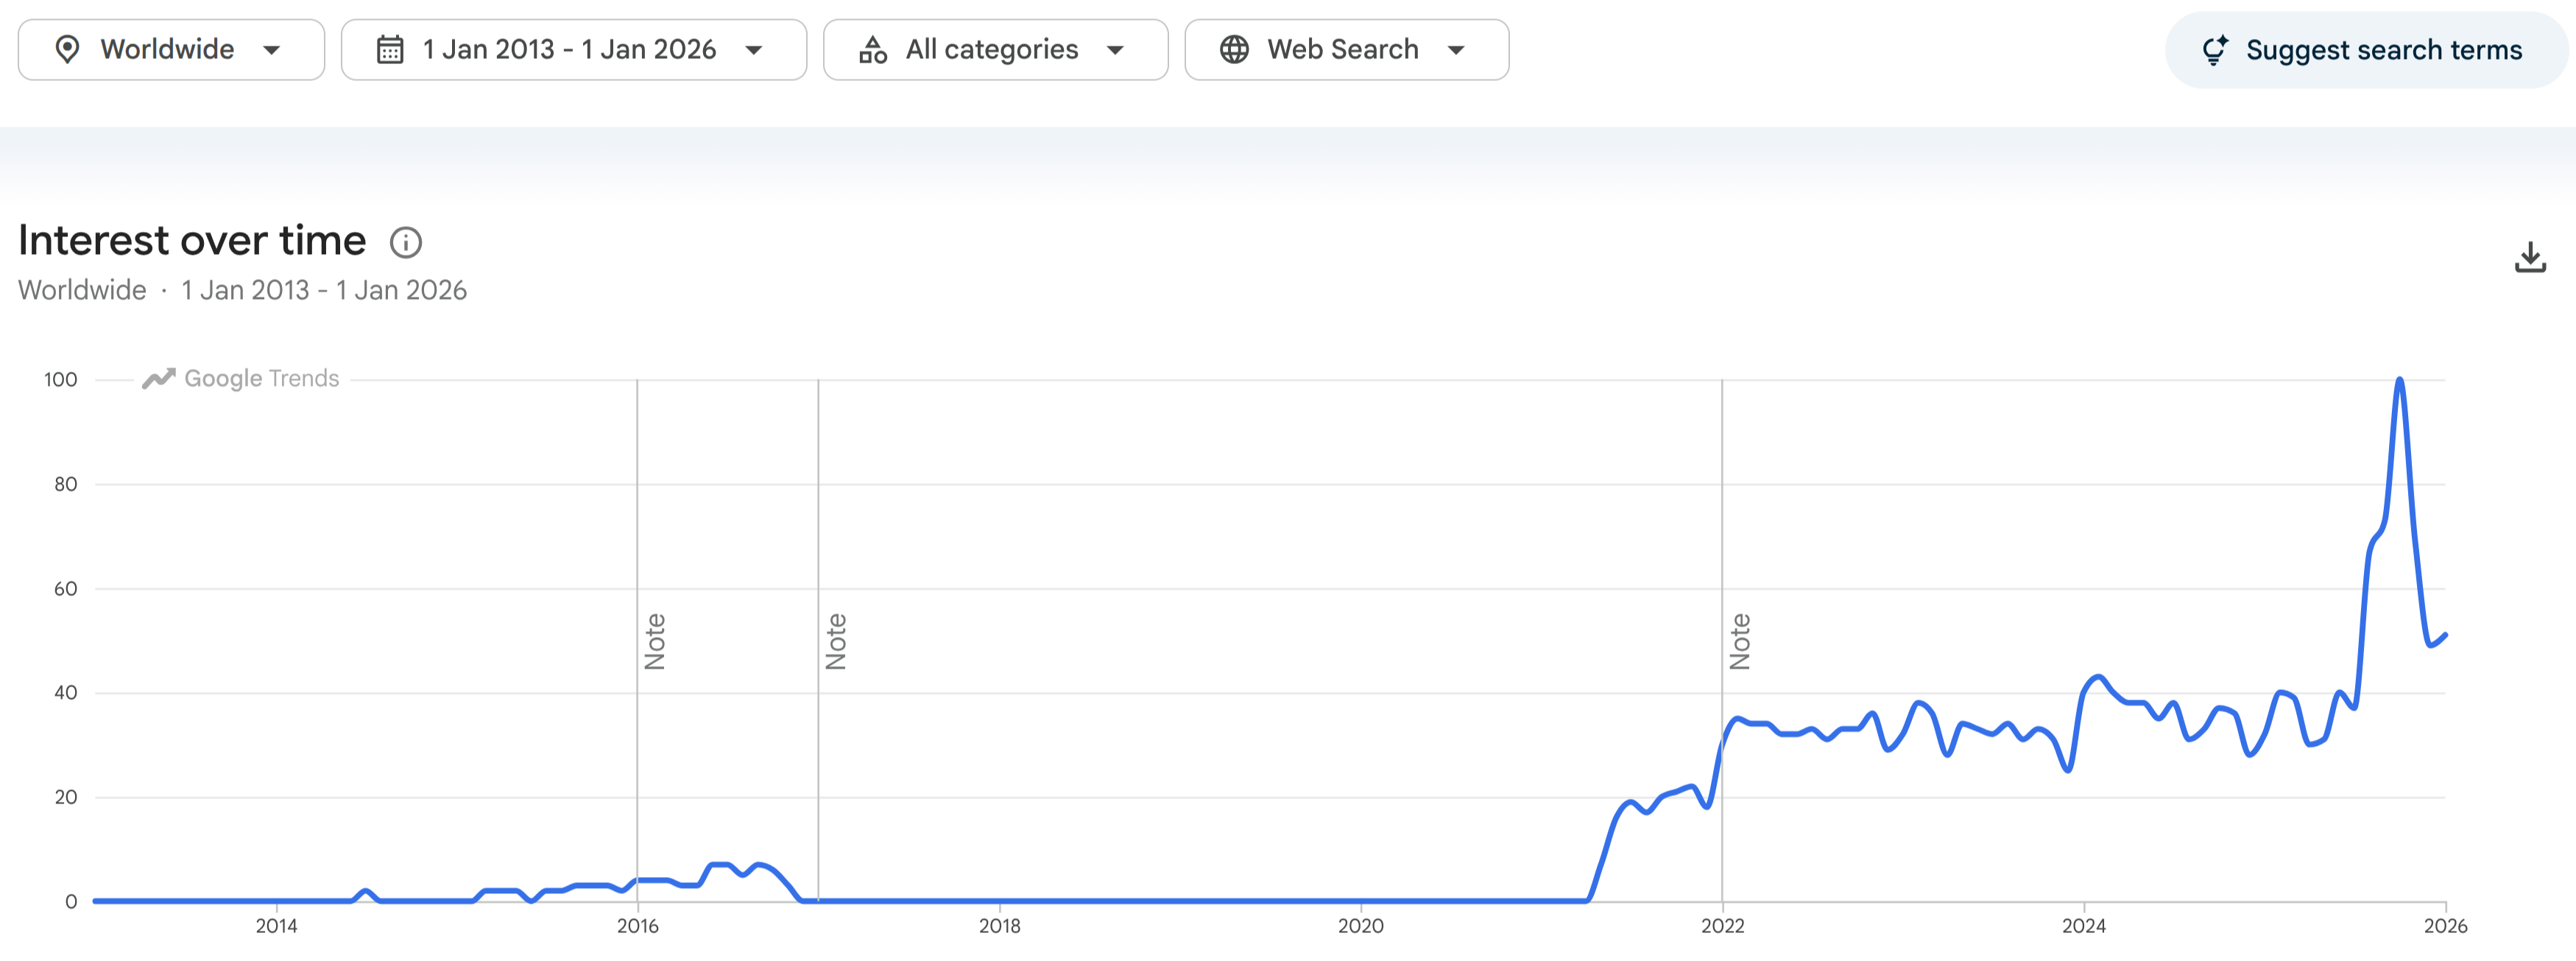
\includegraphics[width=\linewidth]{intro/google-trends}}}
\end{figure}

\end{frame}


%%%%%%%%%%%%%%%%%%%%%%%%%%%%%%%%%%%%%%%%%%%%%%%%%%%
\begin{frame}

\frametitle{Overview}

\begin{itemize}
  \item Background to the problem
  \item Basic structure of Snakemake files through working examples
  \item A final ``larger'' example
  \item Some random tips
  \item Summary
    \begin{itemize}
      \item Answers to questions that people have asked me before
    \end{itemize}
\end{itemize}
\vs

If you find these slides useful (or if I am talking too fast...), my last slide has a QR code to these PDF slides.

\end{frame}


